\section{El modelo de las cajas (Box Model)}

Todos los elementos o etiquetas HTML están contenidas dentro de cajas, estas cajas poseen un margen (\textbf{margin}, es transparente), borde (\textbf{border}), \textbf{padding} (relleno, también transparente) y el contenido (\textbf{content}) en sí de la etiqueta, todos estos conceptos poseen propiedades modificables, los cuales son la parte superior (\textbf{top}), inferior (\textbf{bottom}), izquierda (\textbf{left}) y derecha (\textbf{right}), las cuales funcionan siguiendo las manecillas del reloj: top, right, bottom y left. La \textit{Figura \ref{fig: 19}} muestra una representación de este modelo:
\begin{figure}[H]
    \centering
    \caption{El modelo de cajas}
    \label{fig: 19}
    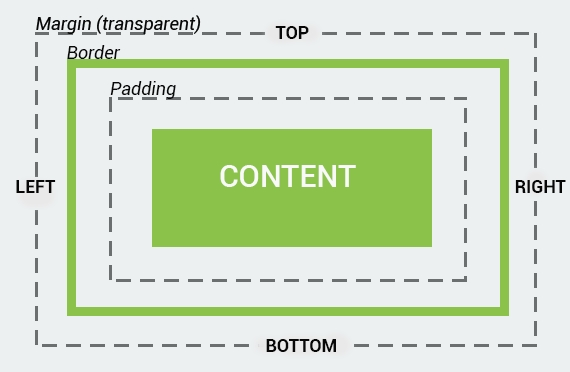
\includegraphics[width=10cm]{ss/box-model.png}
\end{figure}

CSS utiliza este modelo de cajas para determinar su tamaño (ancho y alto) y como colocarlas a lo largo de las páginas del sitio web (considerando el redimensionamiento).


\subsection{Ancho y alto total de un elemento}

Cuando establecemos un ancho para un elemento, este ancho aplica al área de contenido del elemento, pero podemos establecer con CSS el ancho para el padding, margin y border; la \textit{Figura \ref{fig: 20}} contiene un ejemplo de la suma total de todos los anchos del margin, border, padding y content de un elemento:
\begin{figure}[H]
    \centering
    \caption{Ancho total de un elemento}
    \label{fig: 20}
    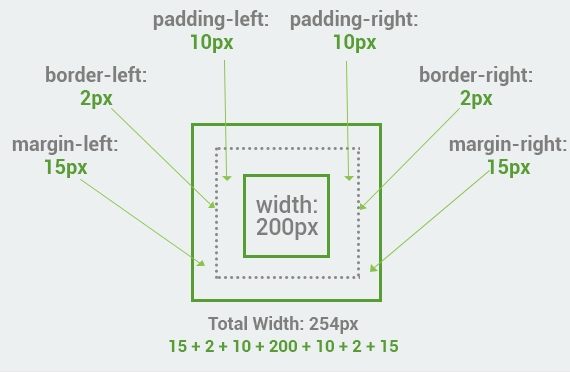
\includegraphics[width=10cm]{ss/box-anchoTotal.png}
\end{figure}

\textit{Nota}: si cambias el background-color de un elemento, este aplica al content y padding del mismo.

Para calcular el alto total de un elemento se sigue el mismo procedimiento que con el ancho, la \textit{Figura \ref{fig: 21}} lo describe:
\begin{figure}[H]
    \centering
    \caption{Alto total de un elemento}
    \label{fig: 21}
    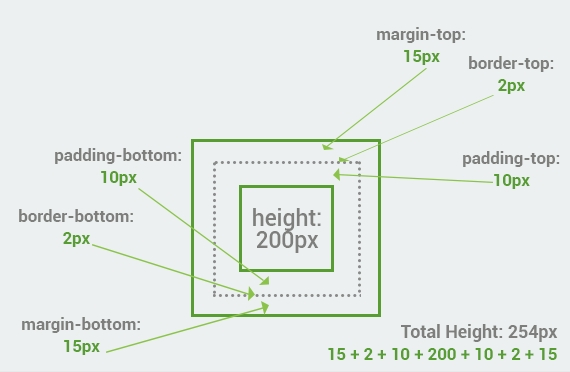
\includegraphics[width=10cm]{ss/box-altoTotal.png}
\end{figure}


\subsection{borders}

La propiedad \textbf{border} de CSS está dividida en tres categorías: \textbf{border-style}, \textbf{border-width} y \textbf{border-color}, para poder definir esta propiedad, se debe establecer un estilo de borde obligatoriamente; se puede establecer en una sola línea con el acceso directo de la propiedad:
\begin{center}
    \textit{
        /* border: grosor estilo color. */ \\
        /* Borde sólido, verde y de grosor de 2 píxeles. */ \\
        border: 2px solid green;
    }
\end{center}

\textit{border-width} puede utilizar \textbf{Longitudes} (\%, px, pt, cm, em, etc.), \textit{border-color} acepta colores pre-establecidos por el lenguaje, además de colores obtenidos a partir de RGB o códigos hexadecimales, y \textit{border-style} tiene algunos valores particulares, los cuales son:
\begin{itemize}
    \item \textbf{none}: sin línea (valor predeterminado).
    \item \textbf{dotted}: línea hecha con puntos.
    \item \textbf{dashed}: línea punteada.
    \item \textbf{double}: dos líneas continuas sólidas.
    \item \textbf{solid}: línea continua sólida.
    \item \textbf{hidden}: similar a \textit{none}, no pone línea, sin embargo, si el elemento tiene una imagen de fondo, el borde tiene un ancho de 0.
    \item \textbf{groove}: borde estilizado con un patrón de colores.
    \item \textbf{ridge}: borde estilizado con el patrón de colores de \textit{groove} invertido.
    \item \textbf{inset}: borde estilizado que da la apariencia de que el elemento tiene profundidad.
    \item \textbf{outset}: borde estilizado que da la apariencia de que el elemento tiene un volumen 3D (contrario a \textit{inset}).
    \item \textbf{inherit}, \textbf{initial} y \textbf{unset}.
\end{itemize}

\textit{Nota}: se puede establecer diferentes estilos a las distintas ubicaciones del borde (border-top-style, border-right-style, border-bottom-style y border-left-style).

A continuación, mostramos un ejemplo de cómo se ve la configuración de un borde en una etiqueta \textbf{p}:
\begin{lstlisting}
    /* Propiedad abreviada. */
    p {
        border: 2px solid green;
    }
    /* Propiedad por separado. */
    p {
        border-width: 3px;
        border-style: double;
        border-color: red;
    }
\end{lstlisting}


\subsection{width \& height}

Las propiedades \textbf{width} y \textbf{height} de CSS modifican el ancho y alto de los elementos HTML respectivamente, estas propiedades aceptan \textbf{Longitudes} (\%, px, pt, cm, em, etc.), lo interesante aquí son las propiedades \textbf{max} y \textbf{min} width o height, que se refieren a el tamaño máximo y mínimo que debe tener un elemento HTML, veamos un ejemplo en código:
\begin{lstlisting}
    p {
        border: 5px solid green;
        min-height: 100px;
        min-width: 200px;
        max-height: 500px;
        max-width: 600px;
    }
\end{lstlisting}


\subsection{background-color}

La propiedad \textbf{background-color} de CSS pinta el fondo de un elemento HTML con un color, el cual puede ser definido mediante los colores predefinidos de CSS, con RGB o códigos hexadecimales:
\begin{lstlisting}
    body {
        background-color: red;
    }
    p {
        color: white;
        background-color: black;
    }
\end{lstlisting}


\subsection{background-image}

La propiedad \textbf{background-image} de CSS establece una imagen como fondo de un elemento HTML, esta imagen puede venir del directorio donde se está trabajando, o de Internet (rutas absolutas o relativas para ambos casos), utilizamos el método \textbf{url()} para enlazar la imagen al fondo del elemento, veamos un ejemplo:
\begin{lstlisting}
    body {
        /* Forma 1: */
        background-image: url("img_dir.jpg");
        /*
        Forma 2: 
        background: url("img_dir.jpg");
        */
    }
\end{lstlisting}

Por defecto, las imágenes se ubican en la esquina superior izquierda del elemento, si esta imagen es más pequeña que el tamaño del elemento, la imagen se repetirá horizontalmente y luego verticalmente, hasta rellenar el elemento.

Podemos establecer más de una imagen como auxiliar, en caso de que la primer imagen establecida no esté disponible u ocurra un error, separando los métodos url por medio de comas (,):
\begin{lstlisting}
    body {
        background-image: url("https://www.infobae.com/new-resizer/Bcx3DWwspJAhUKsx1JccMAeZpZQ=/1200x900/filters:format(webp):quality(85)//s3.amazonaws.com/arc-wordpress-client-uploads/infobae-wp/wp-content/uploads/2018/07/05182149/dogecoin-1.jpg"), url("https://m.media-amazon.com/images/I/51bhb3O7krL._AC_SX425_.jpg");
    }
\end{lstlisting}


\subsection{background-repeat}

La propiedad \textbf{background-repeat} de CSS define como se repetirán las imágenes de fondo de un elemento HTML para rellenarlo, acepta los siguientes valores:
\begin{itemize}
    \item \textbf{repeat}: la imagen se repite horizontal y verticalmente.
    \item \textbf{no-repeat}: la imagen no se repite.
    \item \textbf{repeat-x}: la imagen se repite horizontalmente.
    \item \textbf{repeat-y}: la imagen se repite verticalmente.
    \item \textbf{space}: la imagen se repite dentro del elemento sin sobresalir y ajustando el tamaño de la misma, dejando un espacio blanco uniforme entre cada imagen.
    \item \textbf{round}: similar a \textit{space}, pero no deja espacio en blanco entre imágenes.
    \item \textbf{inherit}, \textbf{initial}, \textbf{round}, etc.
\end{itemize}

Veamos un ejemplo:
\begin{lstlisting}
    body {
        background-image: url("cat.png");
        background-repeat: no-repeat;
    }
    p {
        background-image: url("dog.png");
        background-repeat: inherit;
    }
\end{lstlisting}


\subsection{background-attachment}

La propiedad \textbf{background-attachment} de CSS define si la imagen de fondo se mueve o no junto con el contenido de la página web (scrolling) incluso si el elemento ya tiene una configuración de \textit{scrolleo}, los valores que acepta son:
\begin{itemize}
    \item \textbf{fixed}: la imagen es relativa a la página web que la contiene. Si el elemento tiene un mecanismo de scrolleo, la imagen no se moverá.
    \item \textbf{scroll}: la imagen es relativa al elemento que la contiene. Si el elemento tiene un mecanismo de scrolleo, la imagen no se moverá, sin embargo, el elemento padre (o la misma página web) tienen scrolleo, la imagen se moverá.
    \item \textbf{local}: la imagen es relativa al elemento que la contiene. Si el elemento tiene un mecanismo de scrolleo, la imagen se moverá.
    \item \textbf{inherit}, \textbf{initial}, \textbf{local}, etc.
\end{itemize}

Veamos un ejemplo:
\begin{lstlisting}
    body {
        background-image: url("cat.png");
        background-attachment: fixed;
    }
\end{lstlisting}



\section{Estilizando elementos HTML}


\subsection{Listas}
Con HTML, únicamente existen dos tipos de listas: numeradas y no numeradas, con CSS, podemos aplicar estilos distintos a los puntos o números de ambas listas, siendo estos cuadrados, círculos sin rellenar, números romanos mayúsculos o minúsculos, etc. Podemos cambiar el estilo de ambas listas con la propiedad \textbf{list-style-type}, la cual acepta los siguientes valores:
\begin{itemize}
    \item \textbf{none}: no agrega un punto a la lista.
    \item \textbf{disc}: un círculo rellenado (predeterminado).
    \item \textbf{circle}: un círculo no rellenado.
    \item \textbf{square}: un cuadrado rellenado.
    \item \textbf{decimal}: números decimales, comenzando en 1.
    \item \textbf{lower-roman}: números romanos minúsculos.
    \item \textbf{upper-roman}: números romanos mayúsculos.
    \item \textbf{inherit}, \textbf{initial}, \textbf{unset}, etc. Se pueden aplicar otros tipos de números y letras, tanto mayúsculas como minúsculas, pero los valores anteriores son los más comunes.
\end{itemize}

La propiedad \textbf{list-style-image} permite establecer una imagen como punto de elemento de una lista (se utiliza el método \textit{url()} para definir la imagen), mientras que la propiedad \textbf{list-style-position} fija en qué parte se pondrán los puntos y elementos de las listas (valores \textbf{outside} (predeterminado) e \textbf{inside}).

La propiedad \textbf{list-style} es un acceso directo o forma rápida de usar las tres propiedades anteriormente mencionadas en una sola línea de código; el orden de los valores para esta propiedad son: \textit{type}, \textit{position} y \textit{image}. La \textit{Figura \ref{fig: 22}} muestra un ejemplo:
\begin{lstlisting}
estilos.css
    /*
        Estilo para listas numeradas con número romano mayúsculo,
        sangría regular y sin imagen.
    */
    ol {
        list-style: upper-roman outside none;
    }
    /*
        Estilo para listas no numeradas con cuadrado, mayor
        sangría y con una imagen.
     */
    ul {
        /* Si la imagen no carga, se aplicara el estilo "square". */
        list-style-type: square;
        list-style-position: inside;
        list-style-image: url("point.jpg");
    }

prueba.html
    <!-- Lista no numerada. -->
    <ul>
        <li>Elemento a</li>
        <li>Elemento b</li>
        <li>Elemento c</li>
        <li>Elemento d</li>
    </ul>
    <!-- Lista numerada. -->
    <ol>
        <li>Elemento e</li>
        <li>Elemento f</li>
        <li>Elemento g</li>
        <li>Elemento h</li>
    </ol>
\end{lstlisting}
\begin{figure}[H]
    \centering
    \caption{Propiedades de listas}
    \label{fig: 22}
    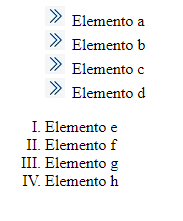
\includegraphics[width=5cm]{ss/lists.png}
\end{figure}


\subsection{Tablas}

Algunas de las propiedades que podemos utilizar para estilizar tablas aparecen en la \textit{Tabla \ref{tab: 3}}:
\begin{table}[H]
    \centering
    \caption{Propiedades para estilizar tablas}
    \label{tab: 3}
    \begin{tabular}{m{3cm} m{5cm} m{5cm}}
        \hline
        \textbf{Propiedad} & \textbf{Definición} & \textbf{Valores} \\
        \hline
        \parbox{3cm}{\textbf{border-collapse}}    & Une (o colapsa) los bordes de las celdas con la de la tabla   & \parbox{4.5cm}{ \textbf{collapsed}: junta los bordes \\ \textbf{separated}: separa los bordes } \\
        \parbox{3cm}{\textbf{border-spacing}}     & Añade espacio vertical y horizontal (comenzando desde la esquina superior izquierda) entre los bordes de celdas con el de la tabla    & \parbox{4.5cm}{ \textbf{Unidades de valores} \\ (px, pt, em, \%, mm, etc.) } \\
        \parbox{3cm}{\textbf{caption-side}}       & Posiciona la \textit{caption} o nombre de la tabla            & \parbox{4.5cm}{ \textbf{top}: pone el título encima de la tabla \\ \textbf{bottom}: pone el título debajo de la tabla } \\
        \parbox{3cm}{\textbf{empty-cell}}         & Dibuja el borde la celda en celdas vacías                     & \parbox{4.5cm}{\textbf{show}: muestra el borde \\ \textbf{hide}: esconde el borde } \\
        \parbox{3cm}{\textbf{table-layout}}       & Define cómo la tabla y el buscador calculará el ancho de columnas dependiendo de su contenido                                         & \parbox{4.5cm}{ \textbf{auto} (predeterminado): calcula el ancho según el contenido de las celdas \\ \textbf{fixed}: toma el ancho de la columna anteriormente fijado } \\
        \hline
    \end{tabular}
\end{table}

La \textit{Figura \ref{fig: 23}} muestra un ejemplo de las propiedades anteriormente mencionadas:
\begin{lstlisting}
estilos.css
    /*
        Clases con las distintas propiedades de tablas.
    */
    table {
        width: 100%;
    }
    .separated {
        border-collapse: separate;
        border-spacing: 20px 15px;
        caption-side: top;
        empty-cells: hide;
        table-layout: auto;
    }
    .collapsed {
        border-collapse: collapse;
        caption-side: bottom;
        empty-cells: show;
        table-layout: fixed;
    }

prueba.html
    <table border="1" class="separated">
        <tr>
            <td width="10%">AAAAAAAAAAAAAAAAA</td>
            <td width="90%">B</td>
        </tr>
        <tr>
            <td>CCCCCCCCCCCCCCCCCCC</td>
            <td>D</td>
        </tr>
        <tr>
            <td>EEEEEEEEEEEEEEEEEEEE</td>
            <td></td>
        </tr>
    </table>
    <br/>
    <table border="1" class="collapsed">
        <tr>
            <td width="10%">FFFFFFFFFFFFFFFFFFF</td>
            <td width="90%">G</td>
        </tr>
        <tr>
            <td>HHHHHHHHHHHHHHHHHHHHHH</td>
            <td>I</td>
        </tr>
        <tr>
            <td>JJJJJJJJJJJJJJJJJJJJJJJJJJJ</td>
            <td></td>
        </tr>
    </table>
\end{lstlisting}
\begin{figure}[H]
    \centering
    \caption{Propiedades de tablas}
    \label{fig: 23}
    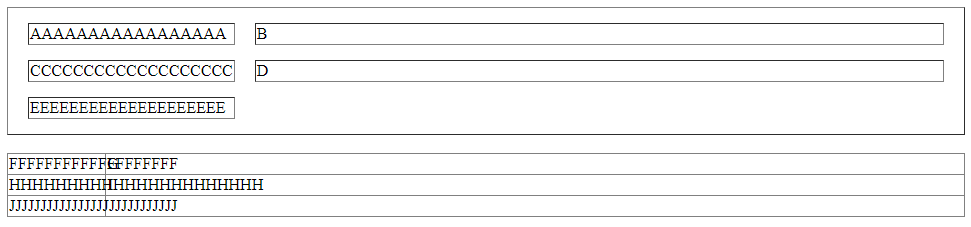
\includegraphics[width=14cm]{ss/tables-border-p.png}
\end{figure}



\subsection{Enlaces}

Se puede estilizar los enlaces según la letra, color de letra o fondo, sin embargo, CSS proporciona pseudo-Selectores adicionales para estilizar un enlace según lo siguiente:
\begin{itemize}
    \item \textbf{a:link}: vista del link sin visitar.
    \item \textbf{a:visited}: vista del link visitado.
    \item \textbf{a:active}: vista del link cuando se le acaba de dar click.
    \item \textbf{a:hover}: vista del link cuando el puntero del mouse está encima.
    \item Existen muchos más pseudo-Selectores, pero los anteriores mencionados son los más utilizados.
\end{itemize}

El orden de la estilización de estos Selectores es el siguiente:
\begin{enumerate}
    \item link.
    \item visited.
    \item hover.
    \item active.
\end{enumerate}


\subsection{Puntero del mouse}

Se puede modificar la apariencia del puntero del mouse bajo ciertas situaciones con CSS. La propiedad a utilizar es \textbf{cursor}, la \textit{Figura \ref{fig: 24}} tiene los siguientes valores (aunque con muchos más):
\begin{figure}[H]
    \centering
    \caption{Valores de ejemplo para \textit{cursor}}
    \label{fig: 24}
    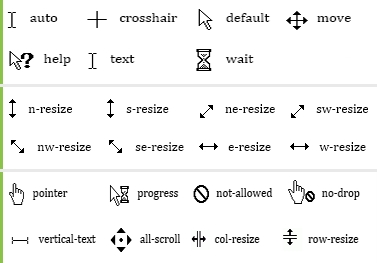
\includegraphics[width=10cm]{ss/cursor.png}
\end{figure}

Entonces, con la propiedad \textbf{cursor} podemos definir, en muchos elementos HTML, la apariencia del puntero del mouse cuando esté está sobre el elemento, se debe seleccionar con cautela su apariencia, debido a que esta le da un indicio al usuario sobre qué está ocurriendo en el sitio, o qué puede hacer cierto componente cuando se le pone el puntero encima.
